% src/slides/source/final/core/04_development.tex

\begin{frame}{Project Development}
  \SlideBody{\begin{VisualCanvas}
    \node[final heading] at (2.4,5.0) {Data};
    \node[final heading] at (7.4,5.0) {Models};
    \node[final heading] at (12.4,5.0) {Evidence};
    \node[inner sep=0pt] at (2.4,3.28)
      {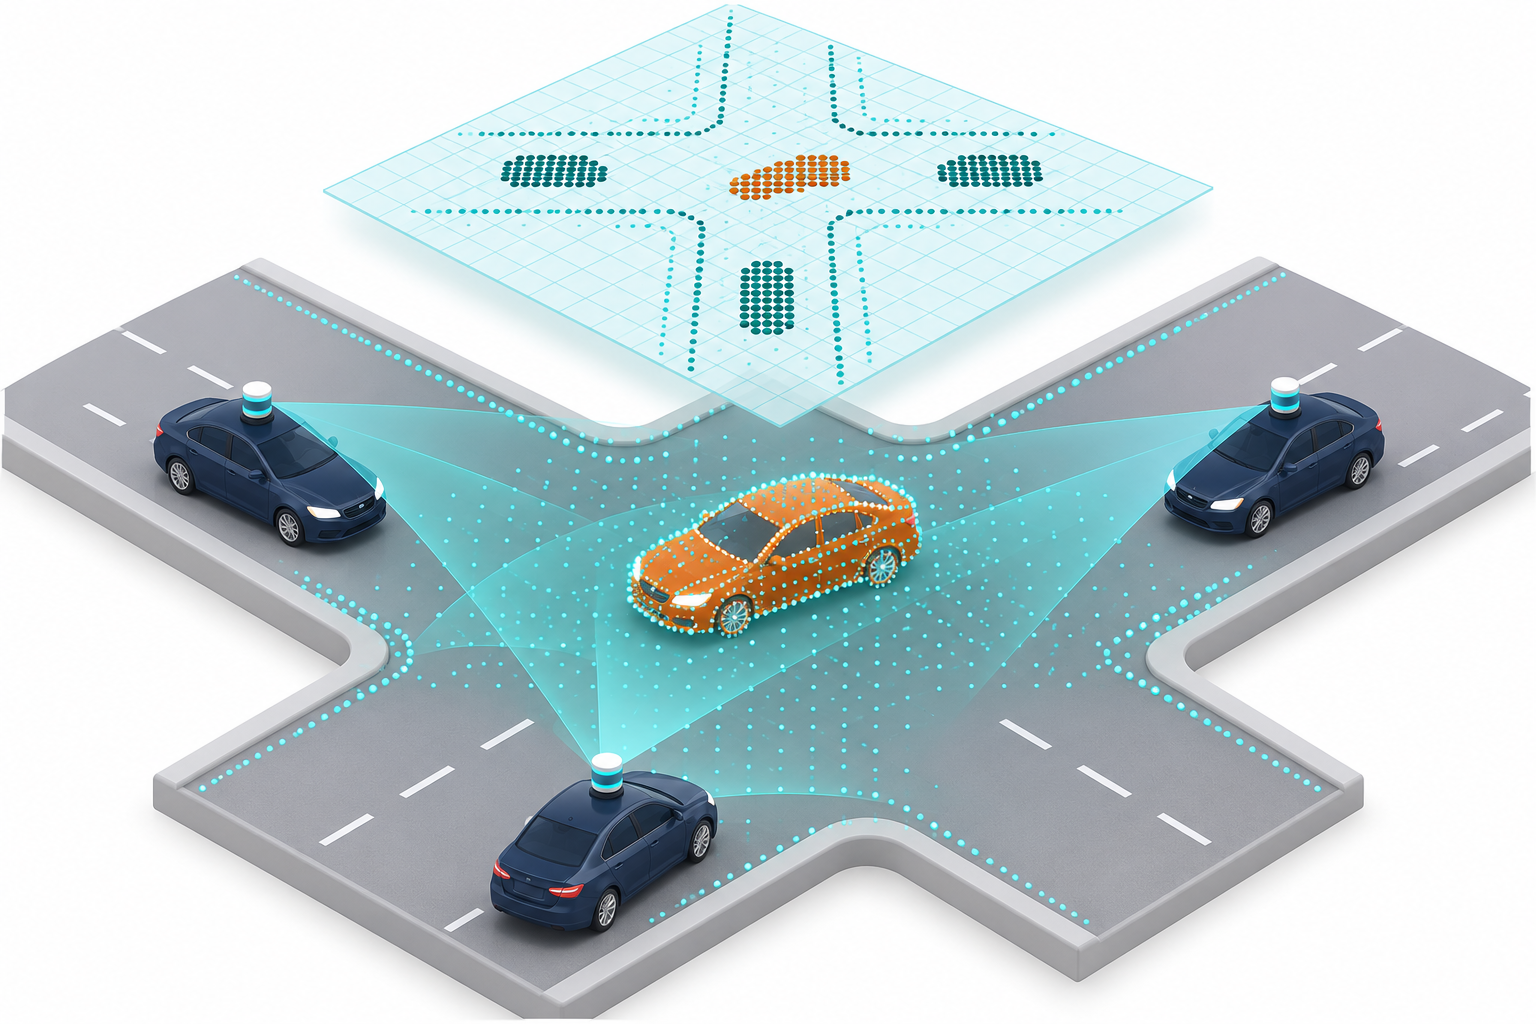
\includegraphics[width=4.0cm,height=2.65cm,keepaspectratio]{assets/illustrations/development/data-imagegen-v1.png}};
    \node[inner sep=0pt] at (7.4,3.28)
      {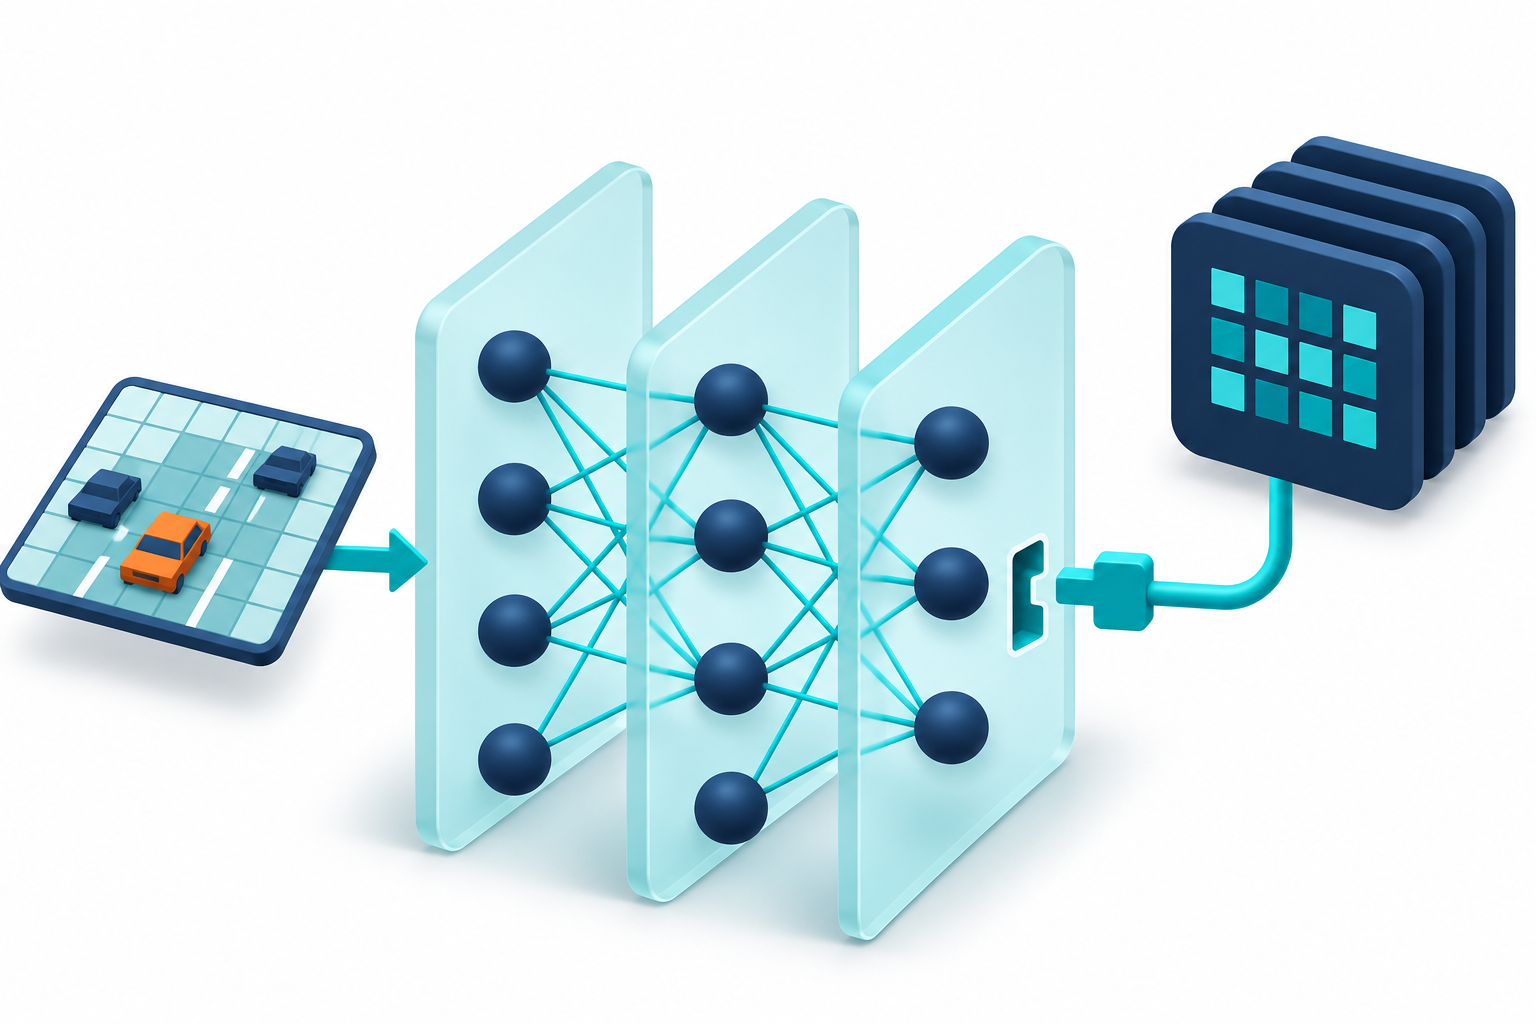
\includegraphics[width=4.0cm,height=2.65cm,keepaspectratio]{assets/illustrations/development/models-imagegen-v1.png}};
    \node[inner sep=0pt] at (12.4,3.28)
      {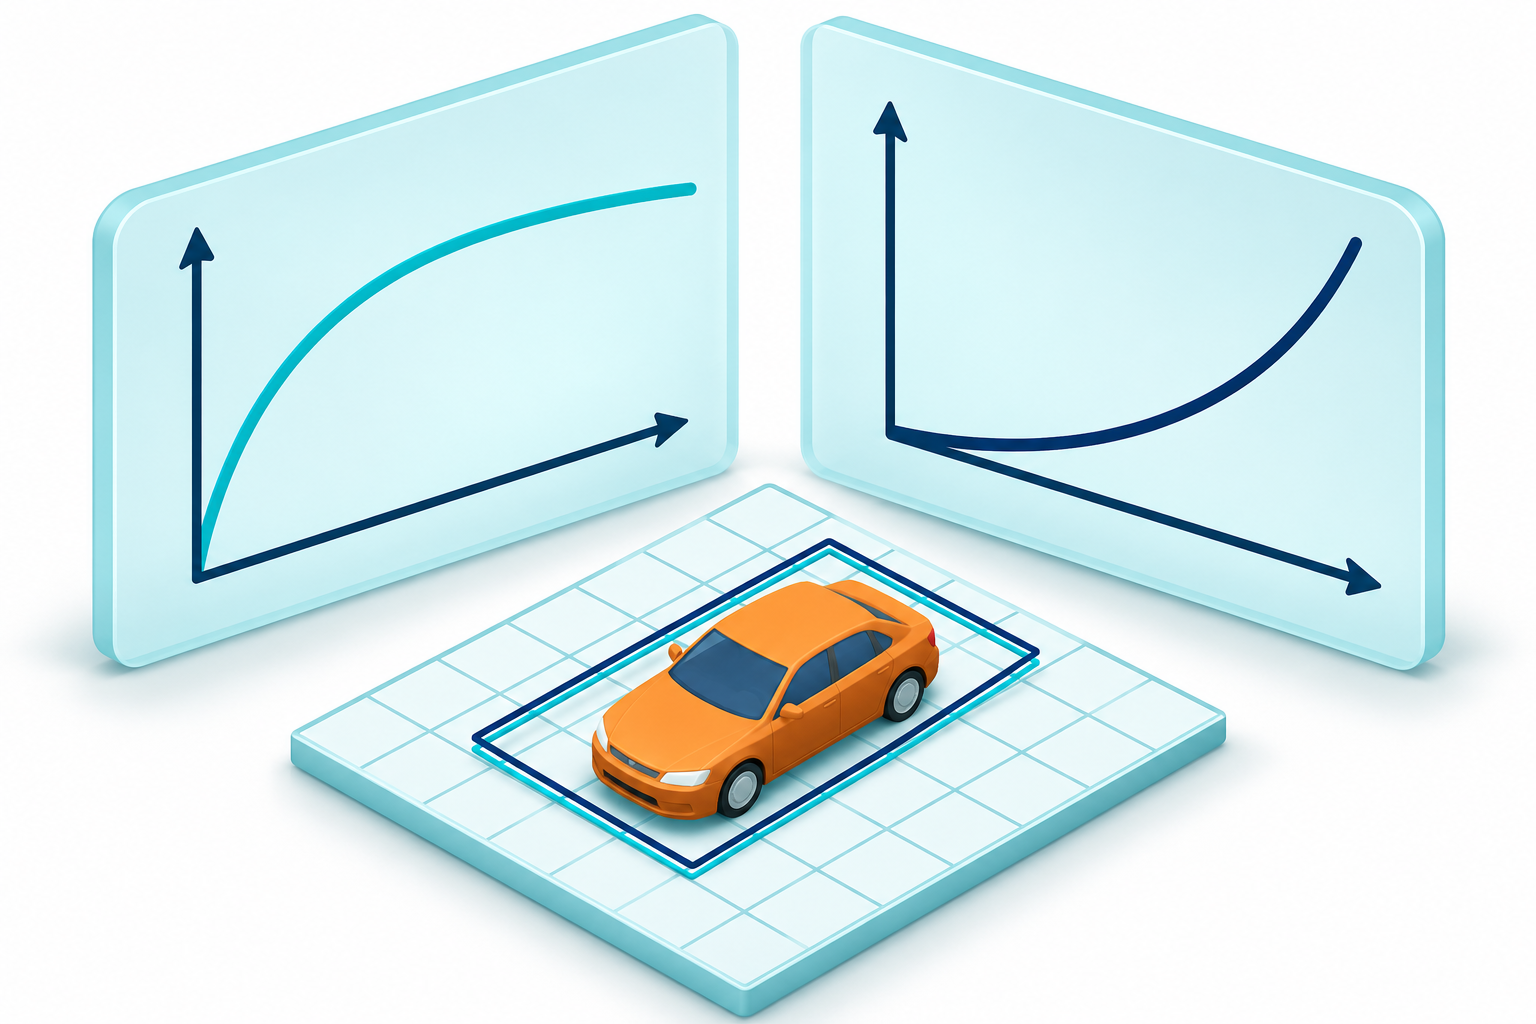
\includegraphics[width=4.0cm,height=2.65cm,keepaspectratio]{assets/illustrations/development/evidence-imagegen-v1.png}};
    \draw[visual arrow] (4.55,3.28) -- (5.25,3.28);
    \draw[visual arrow] (9.55,3.28) -- (10.25,3.28);
    \node[final caption] at (2.4,1.65) {V2X-Sim 2.0};
    \node[final caption] at (7.4,1.65) {Compatible Checkpoints};
    \node[final caption] at (12.4,1.65) {AP + Scaling Curves};
  \end{VisualCanvas}}
  \SlideSource{Source: AI generated illustrations.}
\end{frame}
